
\documentclass[a4paper,12pt]{book}
\usepackage[font=scriptsize]{caption}
\usepackage[T1]{fontenc}
\usepackage[italian,english]{babel}
\usepackage[utf8]{inputenc}
\usepackage{graphicx}
\usepackage{grffile}
\usepackage{color}
\usepackage{float}
\usepackage{cite}
\usepackage{amsmath}
\usepackage{amssymb}
\usepackage{amsthm}
\usepackage{wasysym}
\usepackage{setspace}
\usepackage{algorithm}
\usepackage{algorithmic}
\usepackage{multirow}
\usepackage{listings}
\usepackage{url}
\usepackage[height=21.6cm,width=15cm,centering]{geometry}
\usepackage{tabularx}

\usepackage[bookmarks=true,hyperindex,colorlinks=false,
            pdfborder={0 0 0},pdfstartview=FitH,pdfpagelayout=SinglePage,
            pdfauthor={Marco Edemanti},
            pdftitle={RASD WeatherCal},
            pdfsubject={}]{hyperref}

\title{RASD WeatherCal}
\author{Edemanti Marco}
\author{Polidori Paolo}

\begin{document}
\selectlanguage{english}
\definecolor{lightgray}{rgb}{.9,.9,.9}
\definecolor{darkgray}{rgb}{.4,.4,.4}
\definecolor{purple}{rgb}{0.65, 0.12, 0.82}
\definecolor{lightgreen}{rgb}{0.06,0.60,0.34}
\lstdefinelanguage{alloy}{
  keywords={t assert, pred, all, no, lone, one, some, check, run,
      but, let, implies, not, iff, in, and, or, set, sig, Int, int,
      if, then, else, exactly, disj, fact, fun, module, abstract,
      extends, open, none, univ, iden, seq,},
  keywordstyle=\color{blue}\bfseries,
  ndkeywords={class, export, boolean, throw, implements, import, this},
  ndkeywordstyle=\color{darkgray}\bfseries,
  identifierstyle=\color{black},
  sensitive=false,
  comment=[l]{//},
  morecomment=[s]{/*}{*/},
  commentstyle=\color{lightgreen}\bfseries,
  stringstyle=\color{red}\ttfamily,
  morestring=[b]',
  morestring=[b]"
}
\lstset{ %
  backgroundcolor=\color{white},   % choose the background color; you must add \usepackage{color} or \usepackage{xcolor}
  basicstyle=\footnotesize,        % the size of the fonts that are used for the code
  breakatwhitespace=false,         % sets if automatic breaks should only happen at whitespace
  breaklines=true,                 % sets automatic line breaking
  captionpos=b,                    % sets the caption-position to bottom
  commentstyle=\color{green},    % comment style
  deletekeywords={...},            % if you want to delete keywords from the given language
  escapeinside={\%*}{*)},          % if you want to add LaTeX within your code
  extendedchars=true,              % lets you use non-ASCII characters; for 8-bits encodings only, does not work with UTF-8
  frame=single,                    % adds a frame around the code
  keepspaces=true,                 % keeps spaces in text, useful for keeping indentation of code (possibly needs columns=flexible)
  keywordstyle=\color{blue},       % keyword style
  language=alloy,                 % the language of the code
  morekeywords={*,...},            % if you want to add more keywords to the set
  numbers=left,                    % where to put the line-numbers; possible values are (none, left, right)
  numbersep=5pt,                   % how far the line-numbers are from the code
  showspaces=false,                % show spaces everywhere adding particular underscores; it overrides 'showstringspaces'
  showstringspaces=false,          % underline spaces within strings only
  showtabs=false,                  % show tabs within strings adding particular underscores
  stepnumber=2,                    % the step between two line-numbers. If it's 1, each line will be numbered
  tabsize=2,                       % sets default tabsize to 2 spaces
}
 \begin{center}
    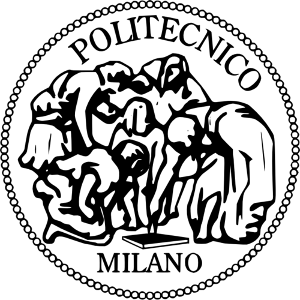
\includegraphics[width=4cm]{../RASD/immagini/polilogo.png}
    \end{center}
\begin{center}

{\huge{\bf\uppercase {Design Documents}}}


\end{center}
\vspace*{0.5cm}
\begin{center}
{\large Project of Software Engineering 2\\ \vspace*{0.5cm} \huge WEATHER-CAL}
\end{center}
\begin{flushright}
 \vspace*{9cm}

        {\bf Authors: }\\
        \vspace*{0.2cm}
            {\bf   {PAOLO POLIDORI} }\\
             \vspace*{0.3cm}
            {\bf   {MARCO EDEMANTI} }
    \end{flushright}

\doublespacing    
\tableofcontents


{\huge Time Reporting}\\ \\
\begin{tabularx}{\linewidth}{|r|X|X|}
  \hline  & {\bf Paolo Polidori} & {\bf Marco Edemanti}\\
  \hline RASD writing & 19 hours & 19 hours\\
  \hline
\end{tabularx}\\
\listoffigures
\lstlistoflistings
\end{document}